%!TEX root = ../../../memoria.tex

\begin{figure}[H]
	\centering
	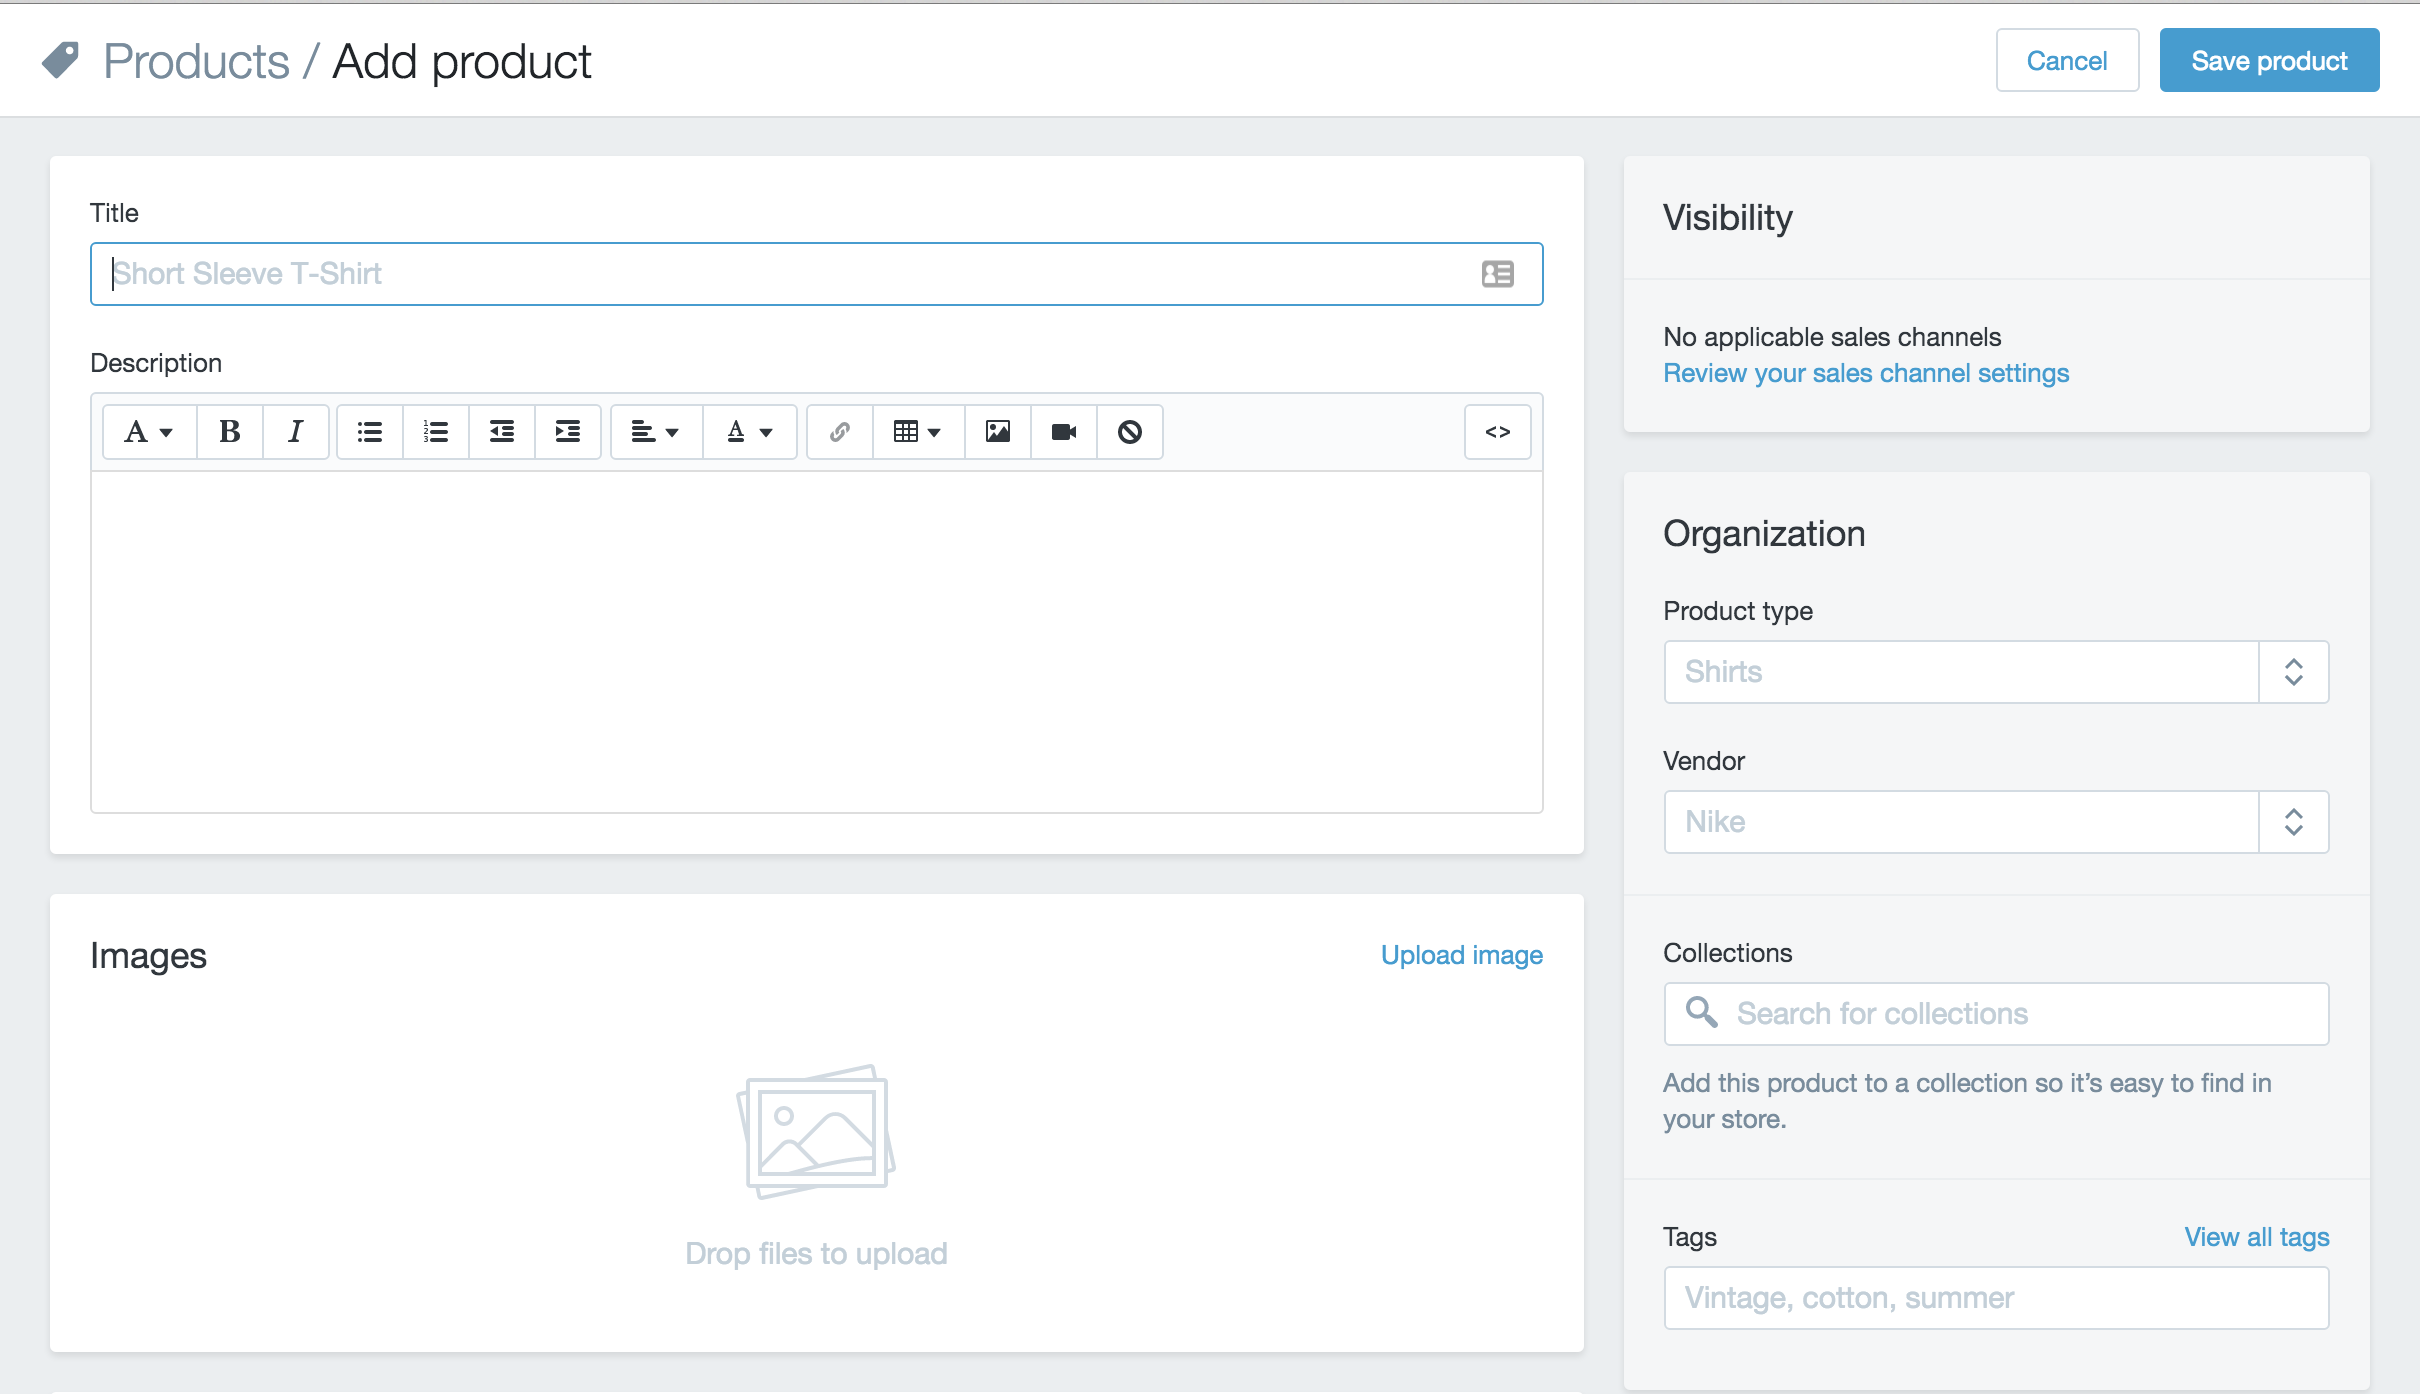
\includegraphics[width=1\textwidth]{figuras/productos/examples/shopify_product_generic_view.png}
	\caption{Formulario de \shopifyNAME para agregar un producto.}
	\label{figure:productos:example:shopify_product_generic_view}
\end{figure}

\begin{figure}[H]
	\centering
	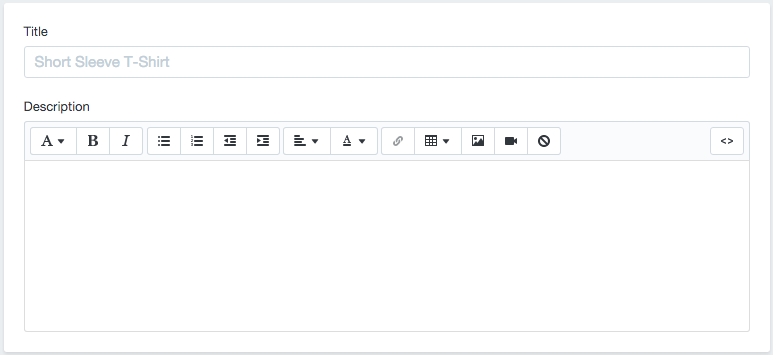
\includegraphics[width=1\textwidth]{figuras/productos/examples/shopify_product_main.png}
	\caption{Sección del formulario de \shopifyNAME para agregar un título y una descripción.}
	\label{figure:productos:example:shopify_product_main}
\end{figure}

\begin{figure}[H]
	\centering
	
\includegraphics[width=1\textwidth]{figuras/productos/examples/shopify_product_multimedia.png}
	\caption{Sección del formulario de \shopifyNAME para agregar imágenes de producto.}
	\label{figure:productos:example:shopify_product_multimedia}
\end{figure}

\begin{figure}[H]
	\centering
	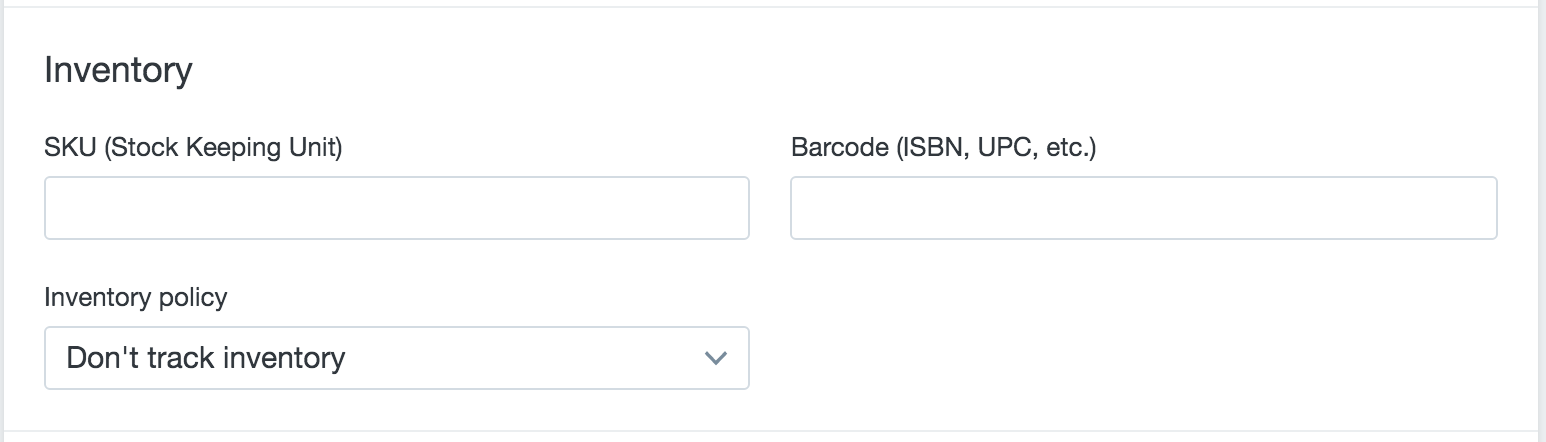
\includegraphics[width=1\textwidth]{figuras/productos/examples/shopify_product_inventory.png}
	\caption{Sección del formulario de \shopifyNAME para agregar inventario al producto.}
	\label{figure:productos:example:shopify_product_inventory}
\end{figure}

\begin{figure}[H]
	\centering
	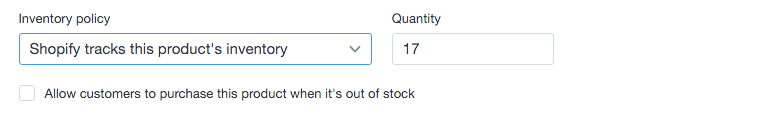
\includegraphics[width=1\textwidth]{figuras/productos/examples/shopify_product_inventory_tracking_enabled.png}
	\caption{Sección \InventoryForm del formulario de \shopifyNAME con opción \trackingForm aceptada.}
	\label{figure:productos:example:shopify_product_inventory_tracking_enabled}
\end{figure}

\begin{figure}[H]
	\centering
	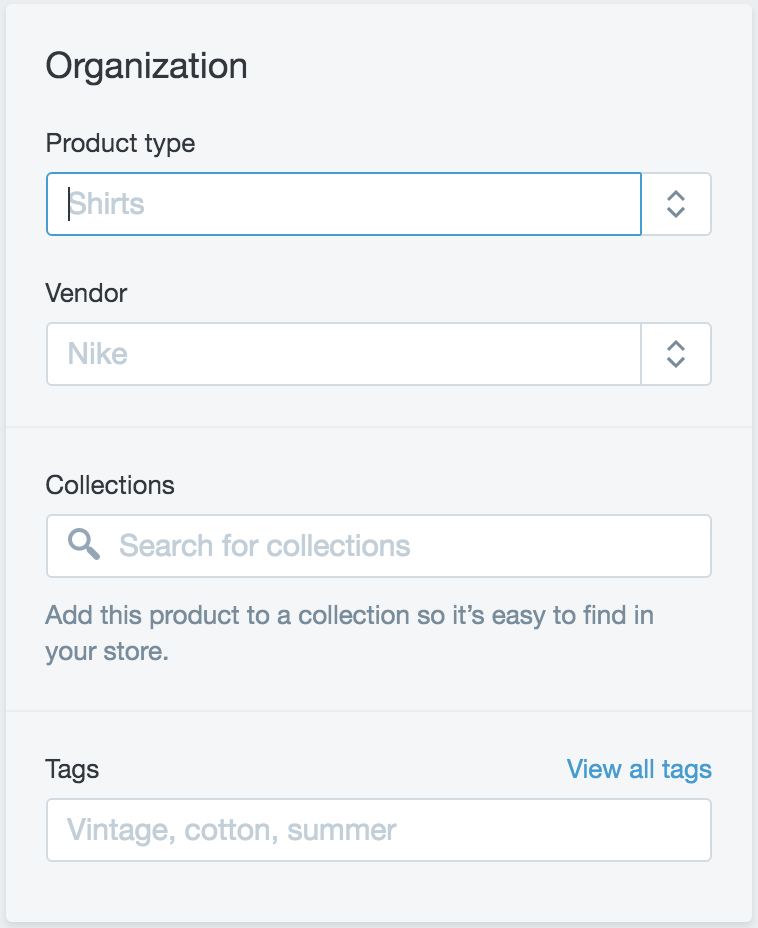
\includegraphics[width=0.6\textwidth]{figuras/productos/examples/shopify_product_organization.png}
	\caption{Sección del formulario de \shopifyNAME para agregar información de la organización del producto.}
	\label{figure:productos:example:shopify_product_organization}
\end{figure}

\begin{figure}[H]
	\centering
	
\includegraphics[width=1\textwidth]{figuras/productos/examples/shopify_product_princing.png}
	\caption{Sección del formulario de \shopifyNAME para agregar información del precio.}
	\label{figure:productos:example:shopify_product_princing}
\end{figure}

\begin{figure}[H]
	\centering
	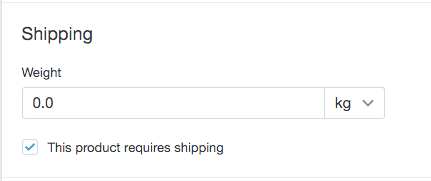
\includegraphics[width=0.6\textwidth]{figuras/productos/examples/shopify_product_shipping.png}
	\caption{Sección del formulario de \shopifyNAME para agregar información de \shipping al producto.}
	\label{figure:productos:example:shopify_product_shipping}
\end{figure}

% \begin{figure}[H]
% 	\centering
% 	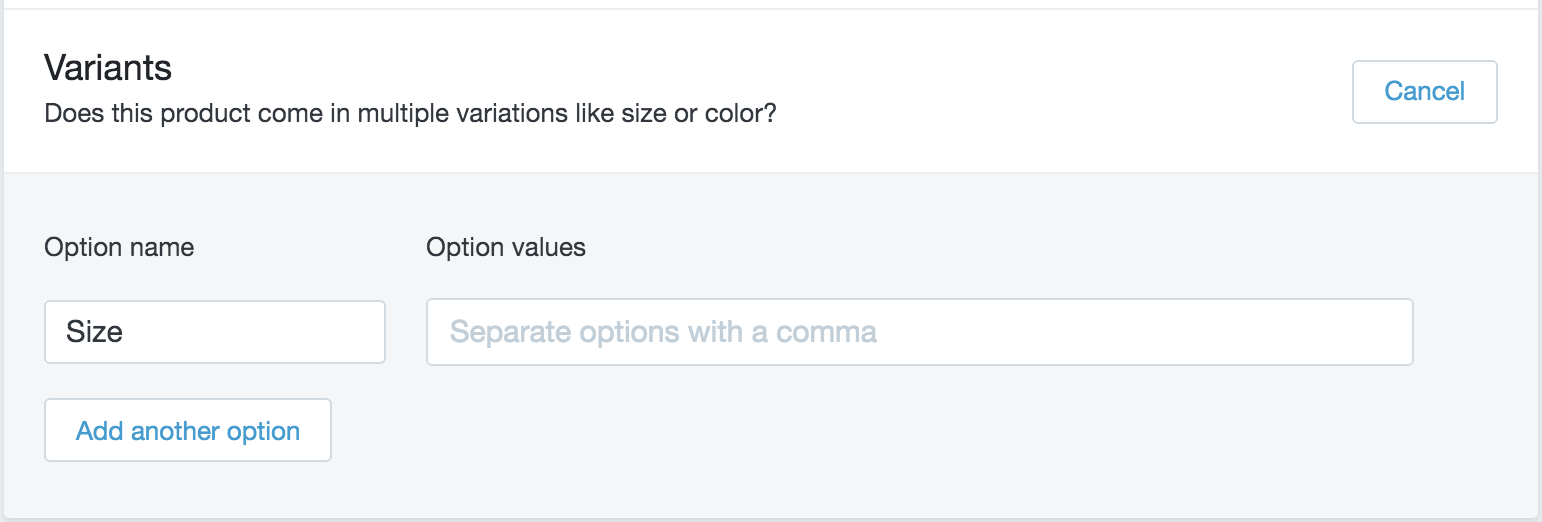
\includegraphics[width=0.9\textwidth]{figuras/productos/examples/shopify_product_variant.png}
% 	\caption{Sección del formulario de \shopifyNAME para agregar variantes.}
% 	\label{figure:productos:example:shopify_product_variant}
% \end{figure}

\begin{figure}[H]
	\centering
	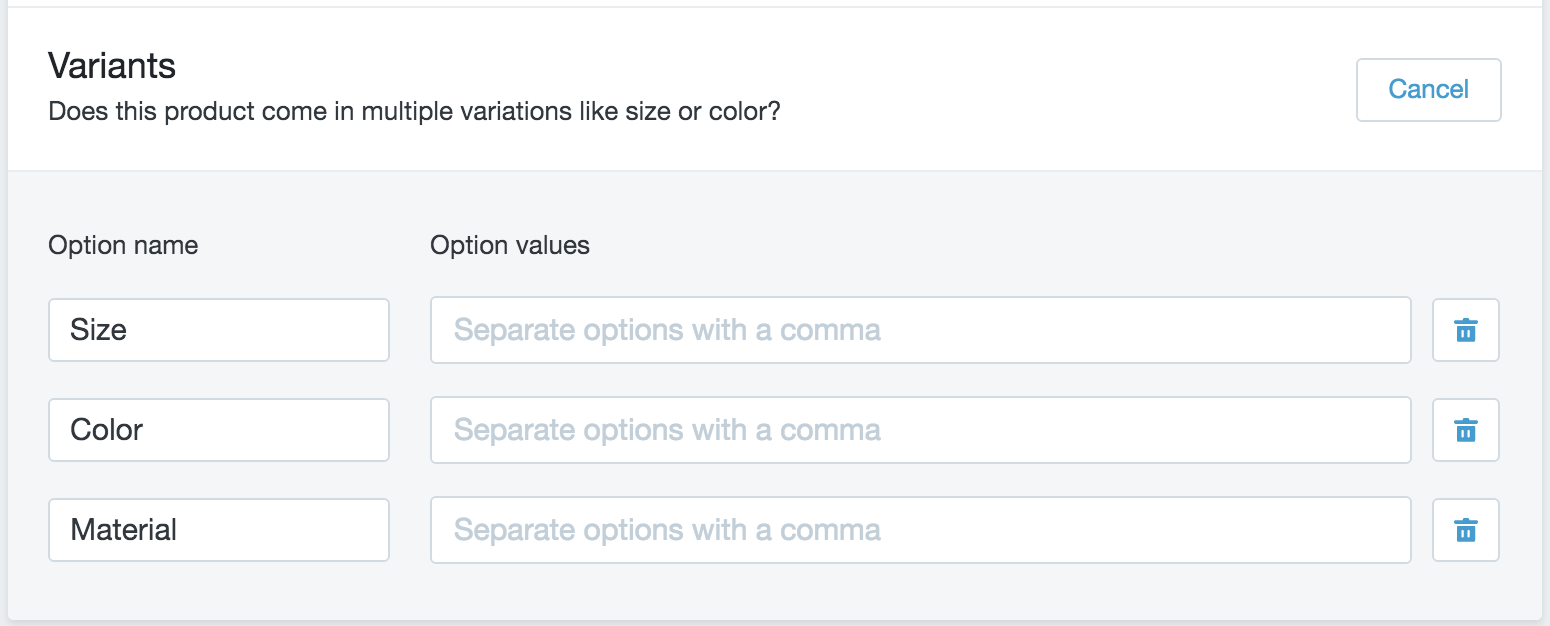
\includegraphics[width=1\textwidth]{figuras/productos/examples/shopify_product_variant_max.png}
	\caption{Sección del formulario de \shopifyNAME para agregar variantes de un producto.}
	\label{figure:productos:example:shopify_product_variant_max}
\end{figure}

\begin{figure}[H]
	\centering
	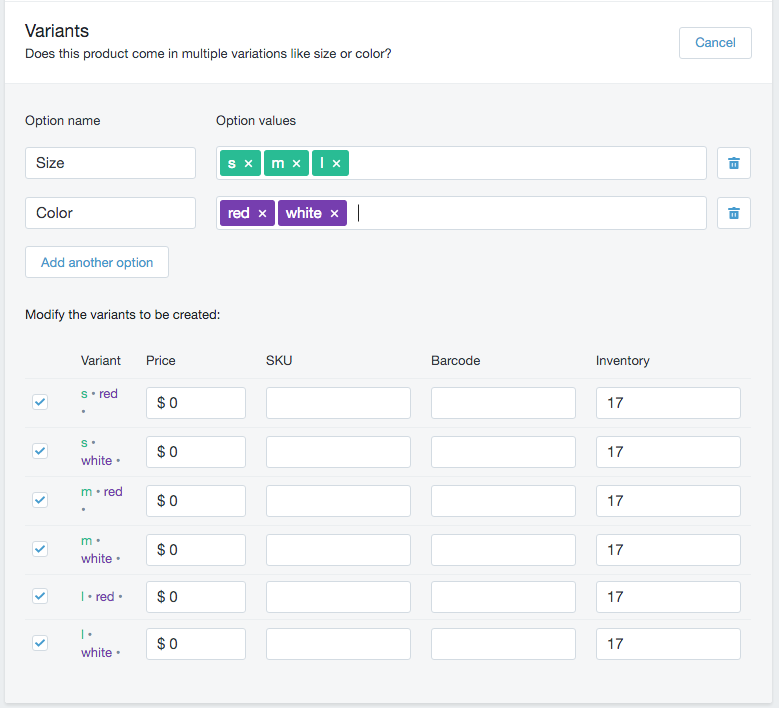
\includegraphics[width=1\textwidth]{figuras/productos/examples/shopify_product_variant_with_info.png}
	\caption{Sección \VariantsForm del formulario de \shopifyNAME con dos variantes del producto.}
	\label{figure:productos:example:shopify_product_variant_with_info}
\end{figure}

\begin{figure}[H]
	\centering
	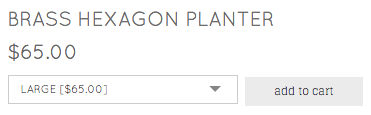
\includegraphics[width=0.6\textwidth]{figuras/productos/examples/leifshop_product_section_add_to_cart.png}
	\caption{Sección del \websiteINT de \leifShopNAME para agregar elementos al carro.}
	\label{figure:productos:example:leifshop_product_section_add_to_cart}
\end{figure}

\begin{figure}[H]
	\centering
	
\includegraphics[width=0.6\textwidth]{figuras/productos/examples/shopify_product_visibility.png}
	\caption{Sección \VisibilityForm del formulario de \shopifyNAME del producto.}
	\label{figure:productos:example:shopify_product_visibility}
\end{figure}

